
\begin{figure}
    \centering
    \begin{subfigure}[c]{0.48\linewidth}
        \centering
        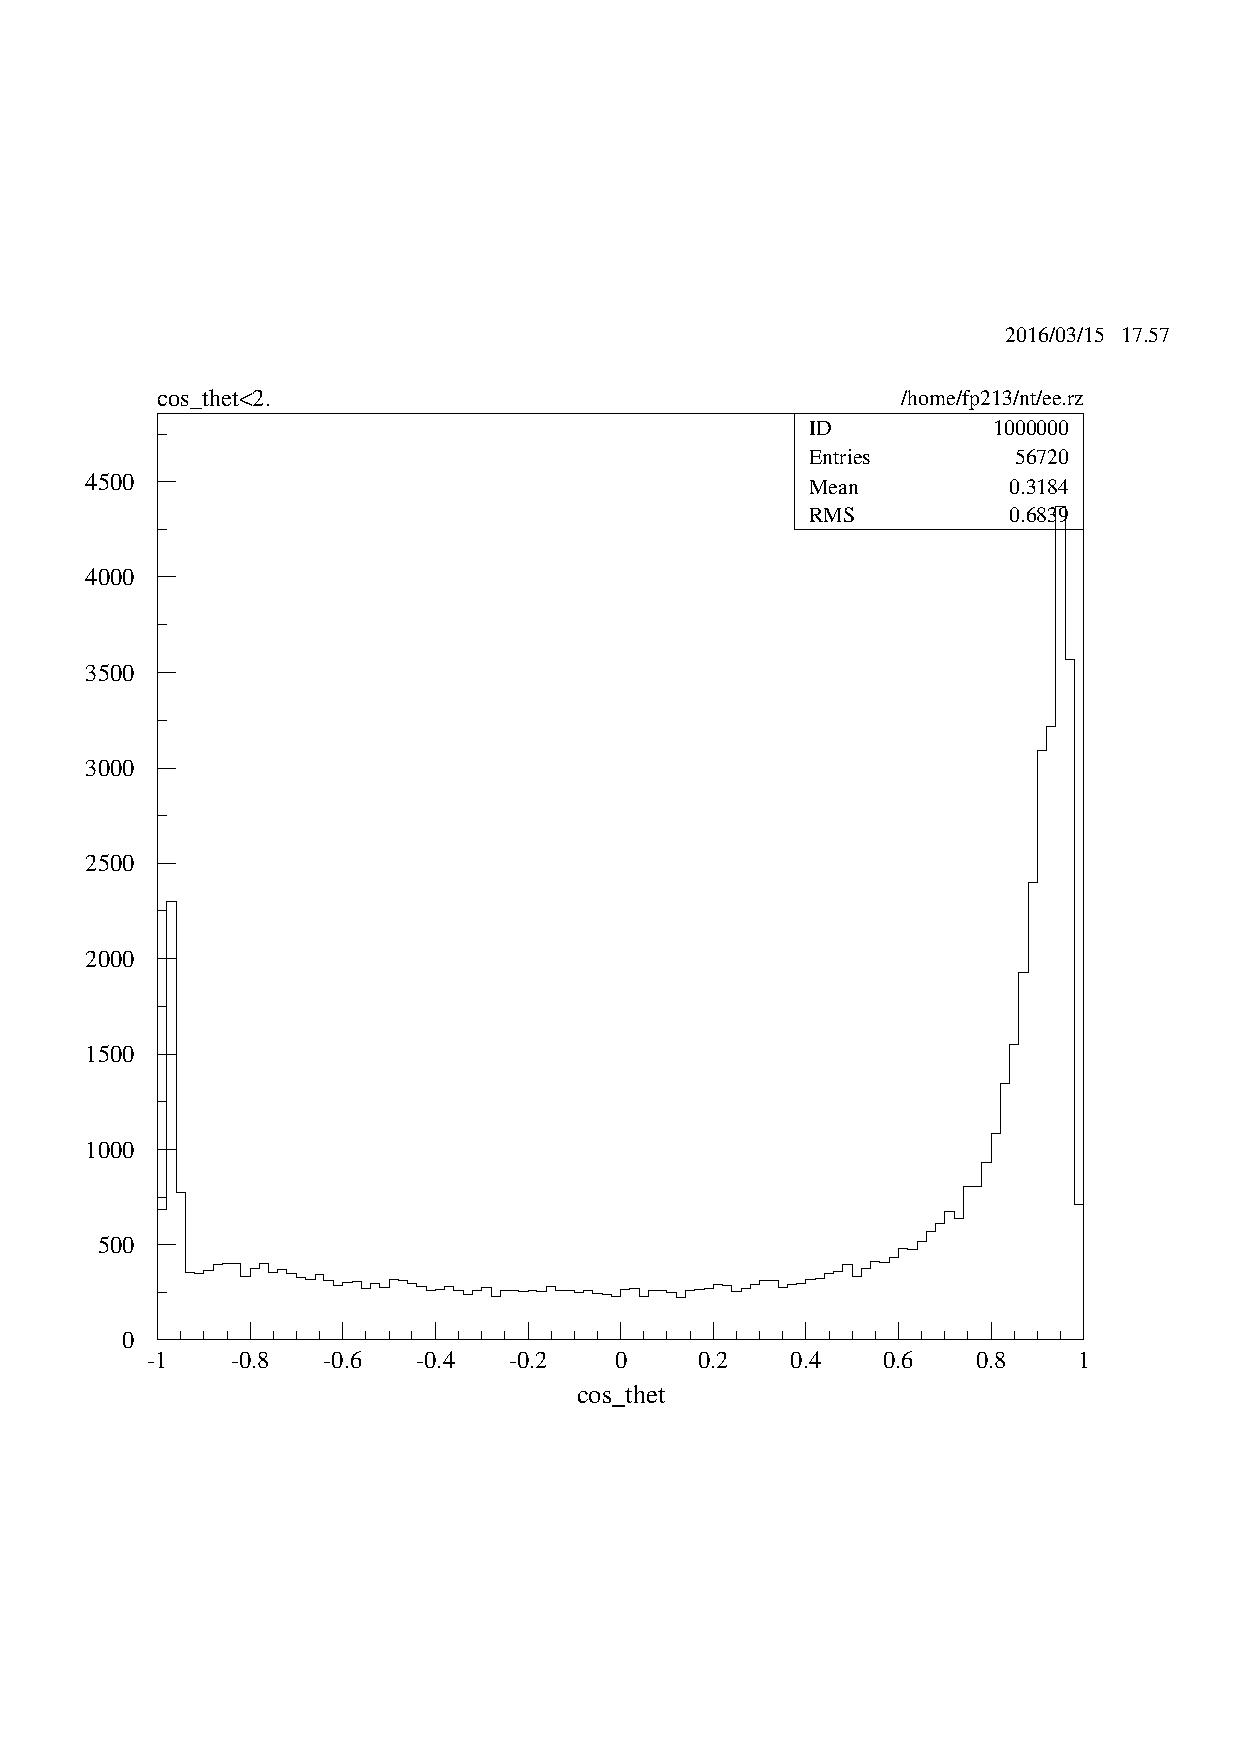
\includegraphics[width=\linewidth]{electrons-cos_thet}
        \caption{%
            Electrons
        }
        \label{fig:paw-angle/electrons}
    \end{subfigure}
    \hfill
    \begin{subfigure}[c]{0.48\linewidth}
        \centering
        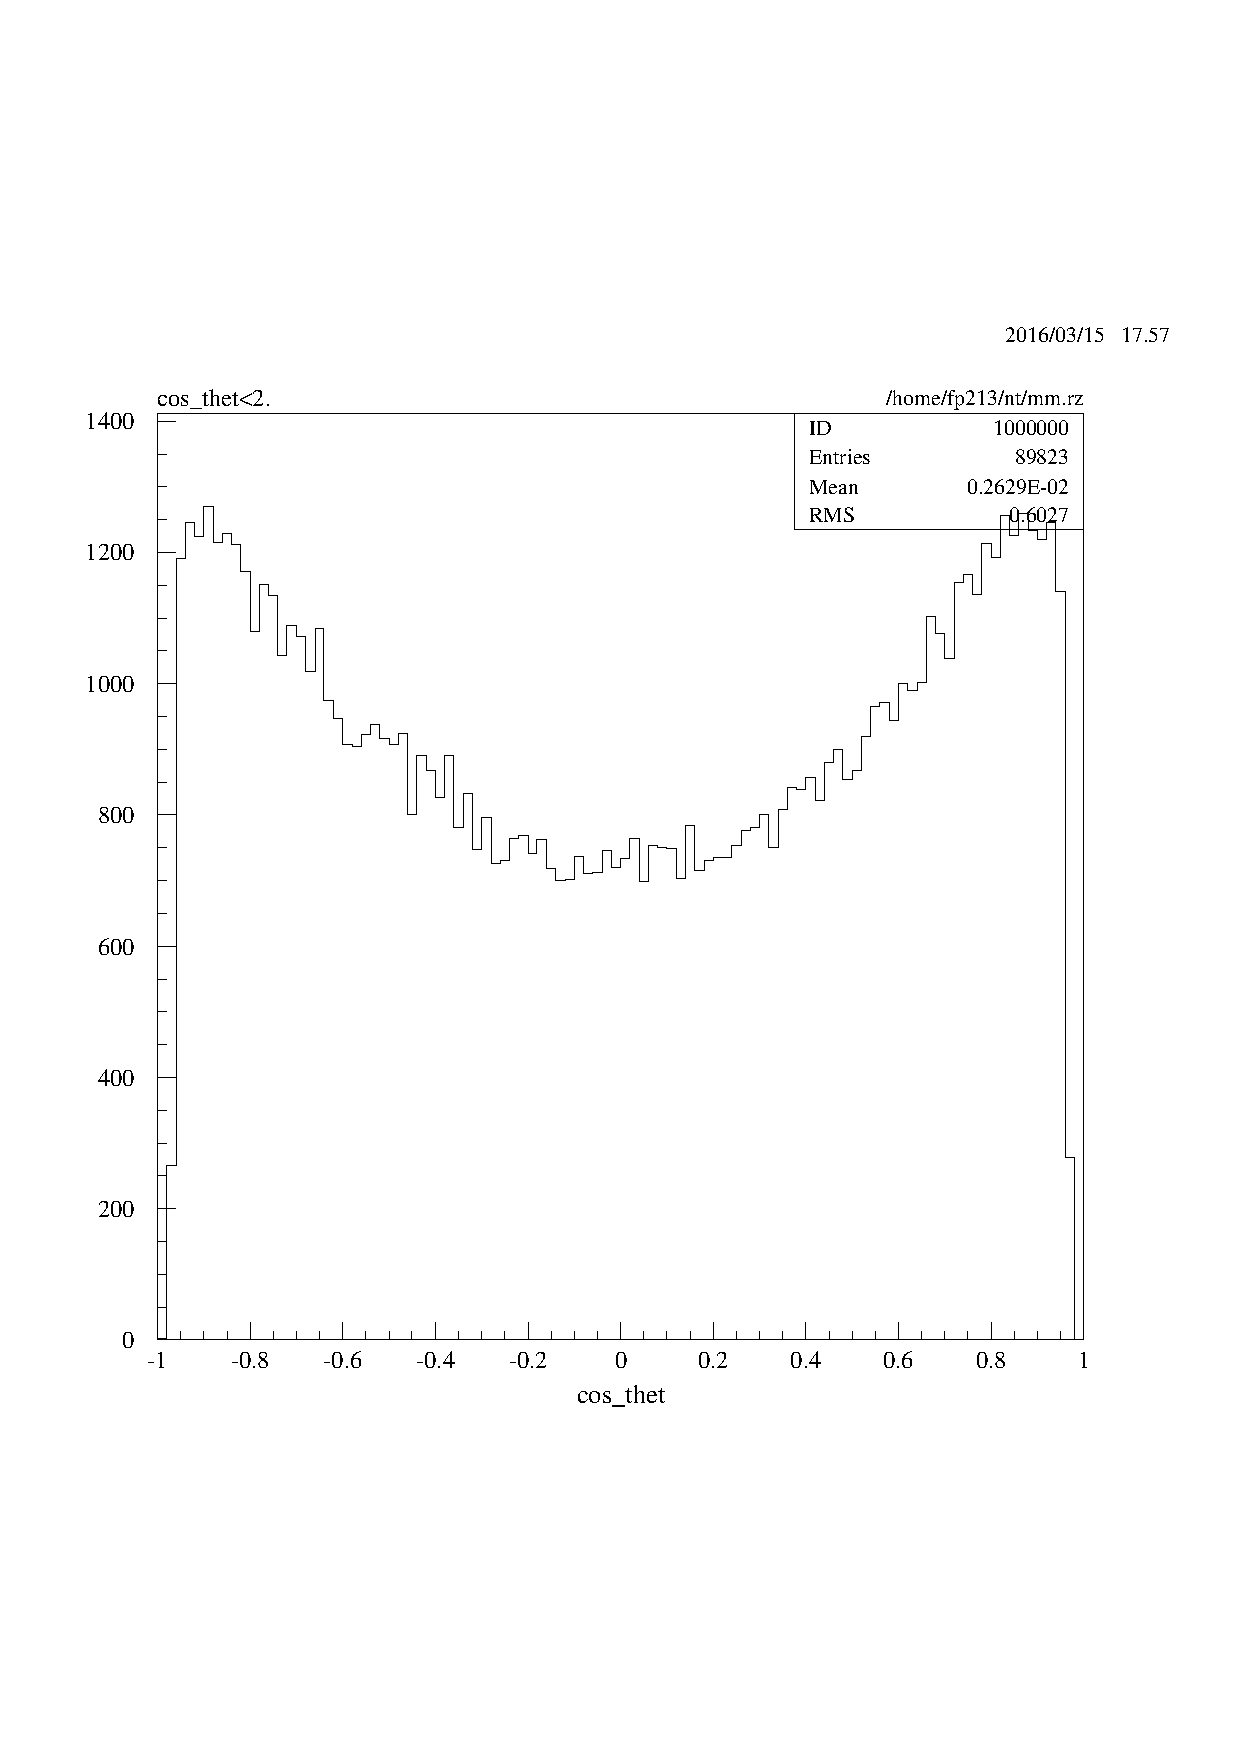
\includegraphics[width=\linewidth]{muons-cos_thet}
        \caption{%
            Muons
        }
        \label{fig:paw-angle/muons}
    \end{subfigure}

    \vspace{2ex}

    \begin{subfigure}[c]{0.48\linewidth}
        \centering
        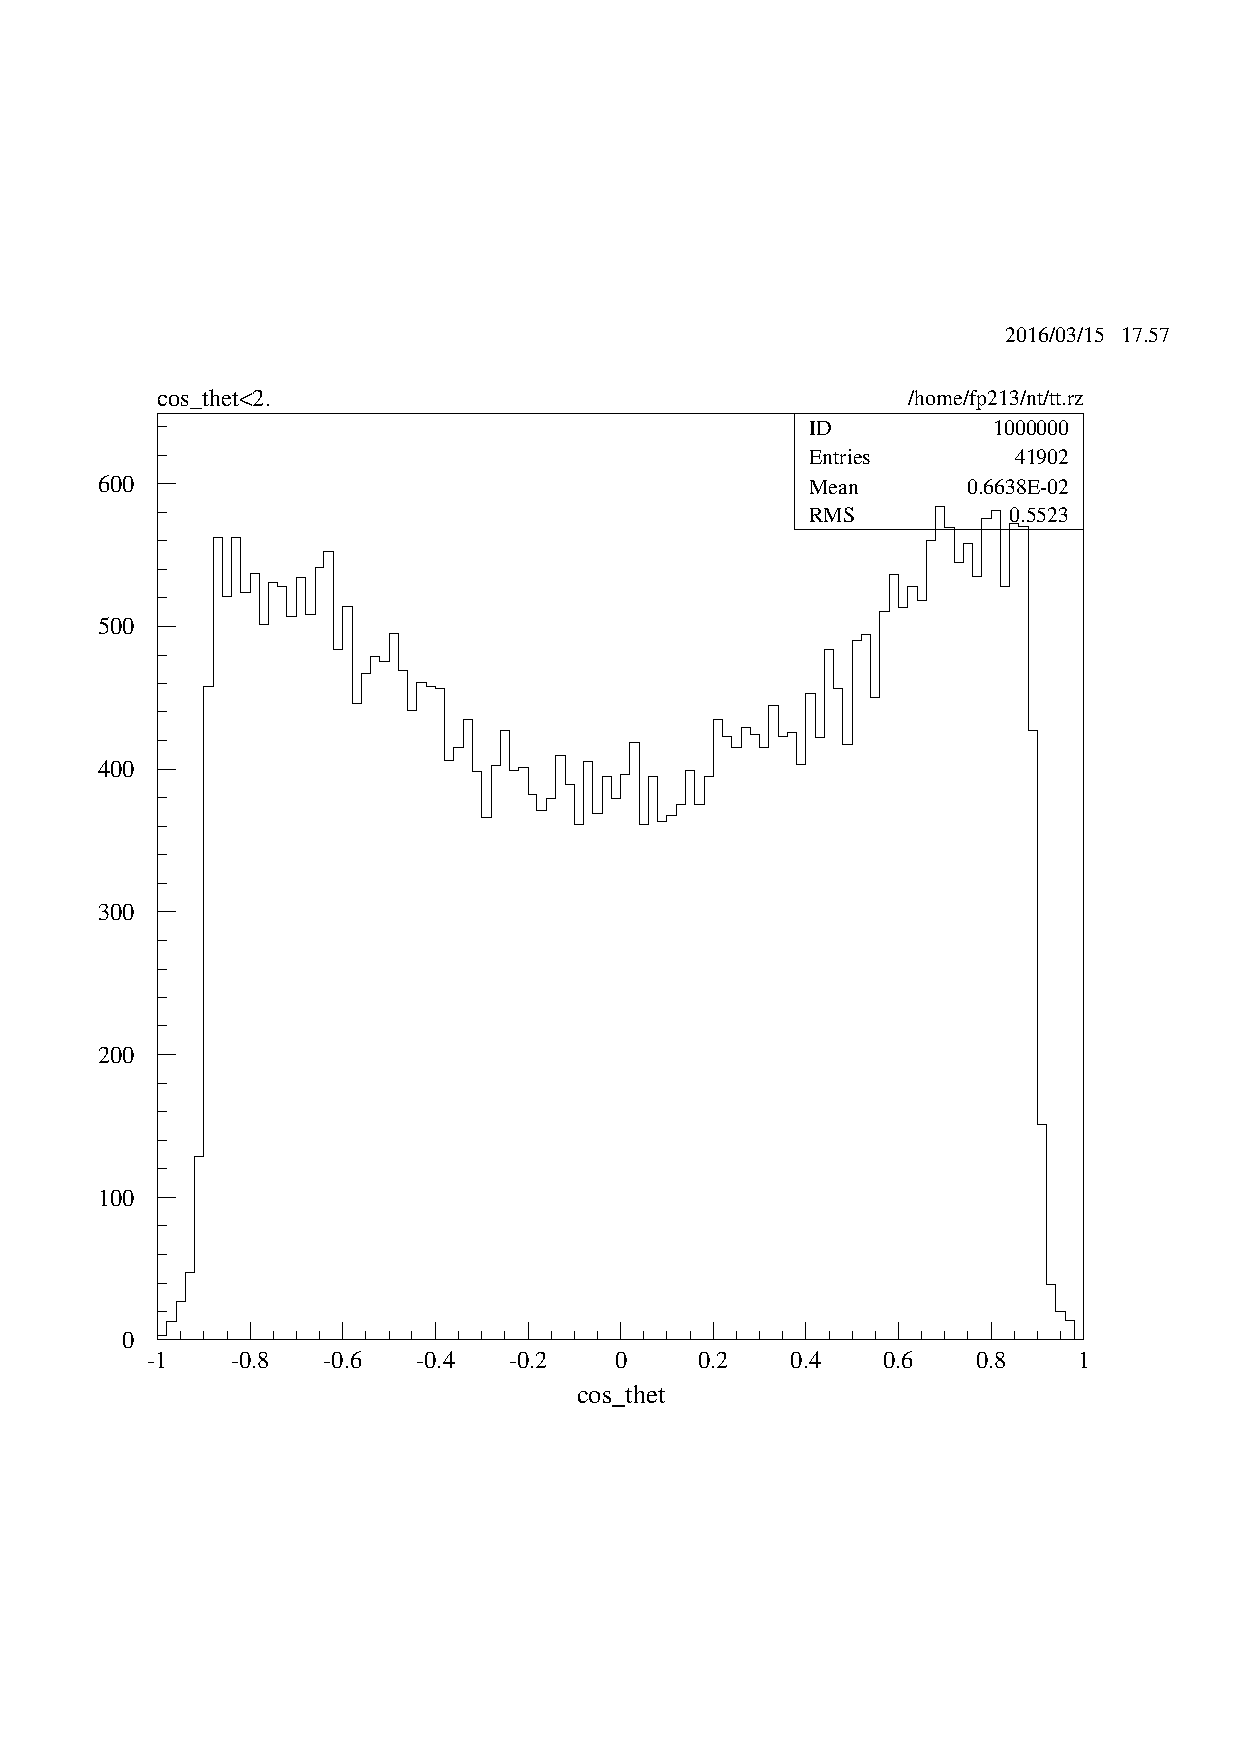
\includegraphics[width=\linewidth]{taus-cos_thet}
        \caption{%
            Tauons
        }
        \label{fig:paw-angle/tauons}
    \end{subfigure}
    \hfill
    \begin{subfigure}[c]{0.48\linewidth}
        \centering
        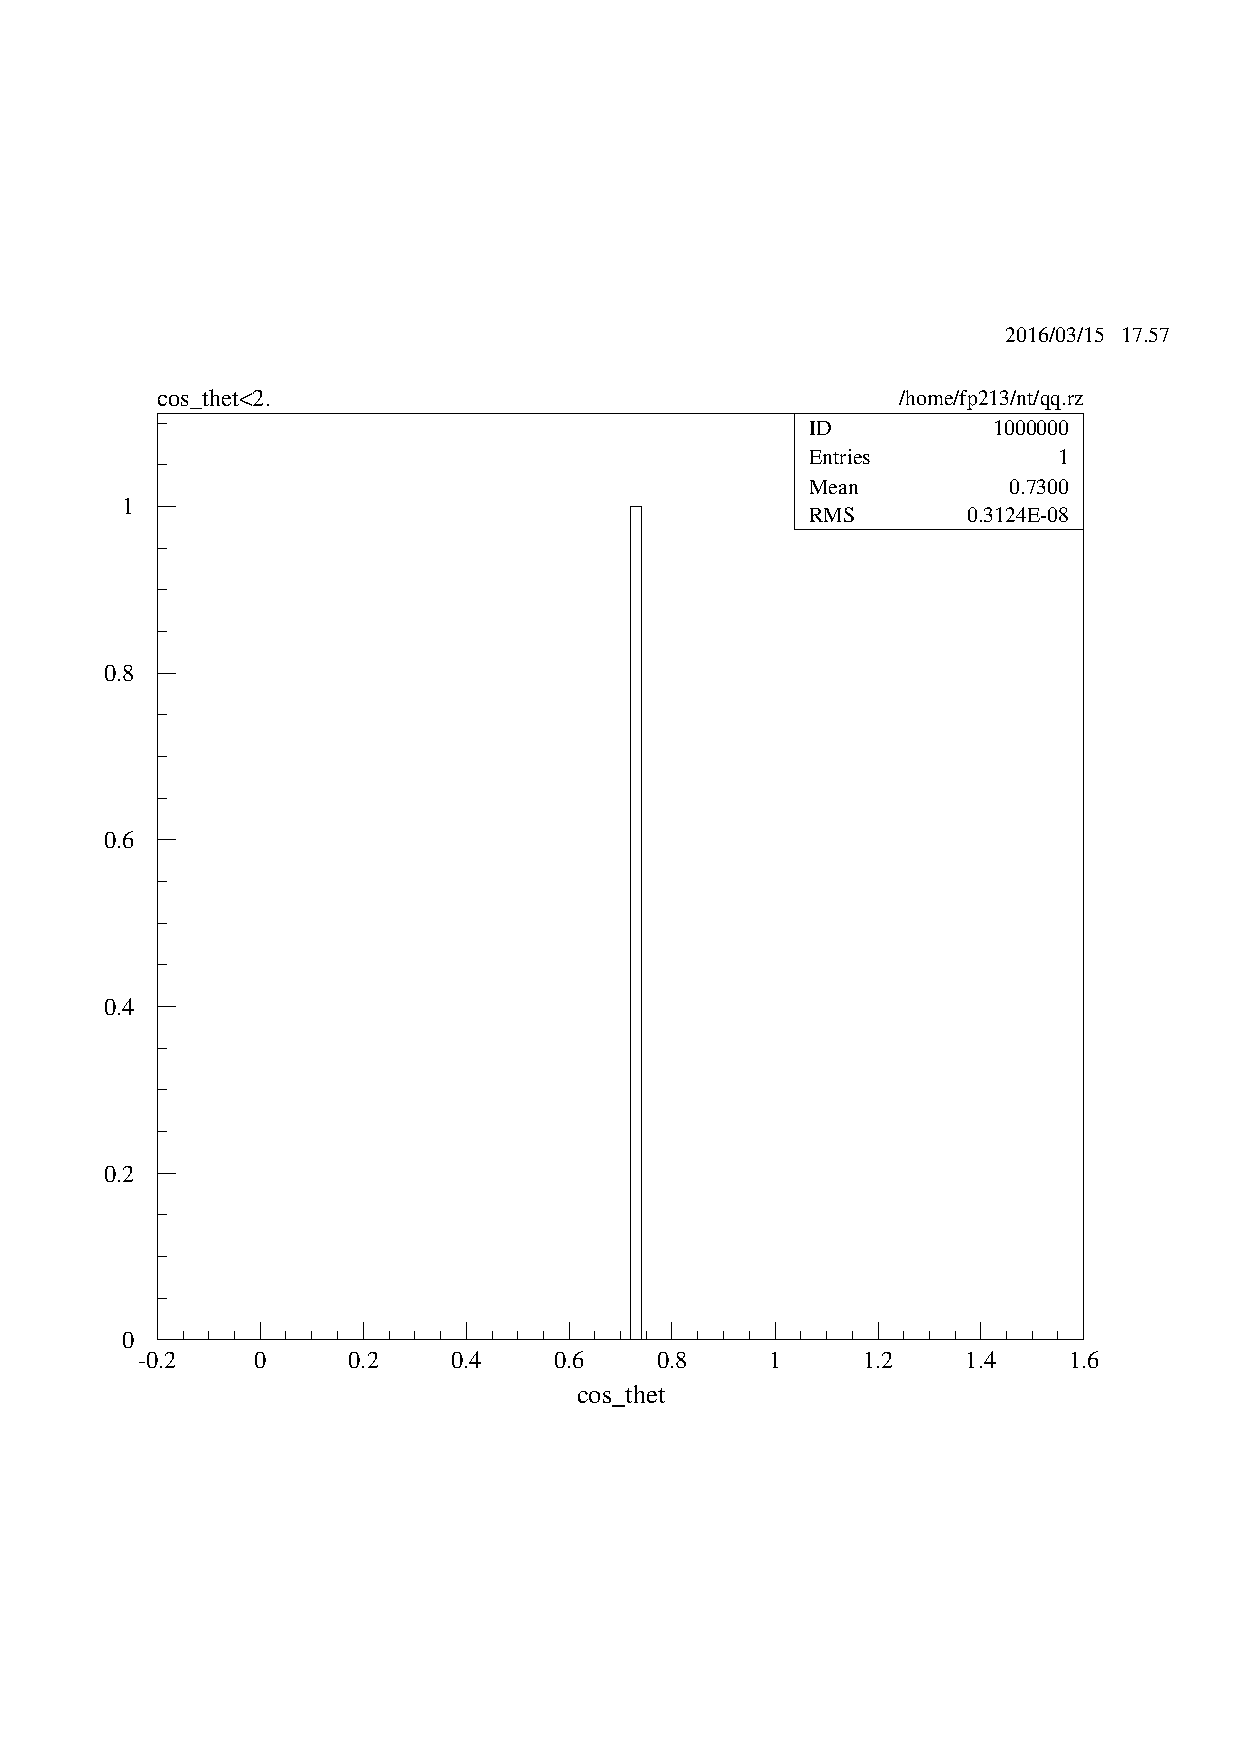
\includegraphics[width=\linewidth]{hadrons-cos_thet}
        \caption{%
            Hadrons
        }
        \label{fig:paw-angle/hadrons}
    \end{subfigure}

    \caption{%
        Angular distribution with respect to $\cos(\theta)$ for the four decay
        types. Histograms generated with \textsc{paw} from Monte Carlo
        datasets. Events without a defined angle are excluded, therefore there
        are no events with more or less than one positively charged track
        included.
    }
    \label{fig:paw-angle}
\end{figure}
